\chapter{Malware Analysis}

There are two types of analysis techniques that can be used to fully understand and dissect a malicious piece of code:

\textbf{Static Analysis} is the process of analyzing a, possibly, malicious piece of software without running it on the machine. This is usually done with the aid of different tools to parse the header of the executable and to extract as many information as possible. Subsequently the malware can be analyzed using a disassembler which is a program that allows the user to take the machine code and "reassemble" it to a higher level, human readable, code. Such process can be taken even further with the use of a decompiler, this software tries to bring a higher level of abstraction into the reversing process by decompiling machine code into a pseudo-language often similar to C reducing the effort required by the analyst to interpret machine code.

This kind of analysis is usually very time consuming and requires deep understanding of the underlying architecture of the processor. Moreover the malware author can use different techniques to modify the compiled code making it harder to reverse engineer or even to trick the analyst into believing that the code has different capabilities than the real ones. These techniques are commonly referred as \textbf{Obfuscation} however there are many different techniques that are used to hide malware capabilities: \textit{Encryption, Packing, Obfuscation, Polymorphism, Metamorphism}.\cite{Ye2017ASO}

\textit{Encryption} and \textit{Obfuscation} are similar techniques used to hide pieces of the malicious code not only from the analyst but also from antivirus software. At low level often \textit{Encryption} consists of performing a \textit{XOR} operation on a defined portion of memory while \textit{Obfuscation} involves masquerading API calls and split strings in the code in order to make it harder to understand the real behaviour of the malware.

On the other hand \textit{Packing} consists in encrypting and compressing the real code of the malware and, instead of shipping the "real" malicious code, the packed version will feature an unpacking stub which will take care of extracting and then running the malware directly into the memory making it harder to detect and reverse engineer.

Finally \textit{Polymorphism} and \textit{Metamorphism} are conceptually similar, the first one involves a polymorpic engine which allows to compile the code in a non deterministic way meaning that it will be different at each compilation but it will however still retain all the initial functionalities, this is usually achieved also with the use of encryption. \textit{Metamorphism} on the other hand is a really interesting technique through which the code of a program can be modified at run time adding a great layer of complexity and opening the door to a dedicated category of malware.

The Static Analysis is an powerful technique however for some more advanced pieces of malware it is not enough and instead it is required to run the malicious code in order to fully understand the capabilities and interactions with the machine.

\textbf{Dynamic Analysis} is the process of running the malicious program in a controlled environment, this is usually a virtual machine with proper measures in place to avoid external communication and instead capture and analyze network traffic. Such virtual machines are also equipped with introspection tools such as \textit{process monitor, process explorer, fakenet-ng} and similar allowing the malware analyst to deeply investigate the behaviour of a malicious program.

This kind of analysis involves running the sample with a debugger attached, a debugger allows the analyst to inspect the internal structure of the machine at runtime having direct access to CPU registers, process memory and allowing the user to modify the control flow of a program using breakpoints, inserting custom instructions and modify the memory during execution. 

There are also ad-hoc sandboxes used to automatically run a malware and then collect all the different interactions with the system producing then a detailed report. This is often referred as automatic malware analysis and the most common sandboxes are cuckoo\footnote{\url{https://cuckoosandbox.org/}}, joe sandbox \footnote{\url{https://www.joesandbox.com/}} and VMRay \footnote{\url{https://www.vmray.com/}}. 

In most cases the best analysis technique is a combination of the two. As a matter of fact debuggers are often used to unpack malware by setting breakpoints in the code and running it in a controlled environment until the real malware is extracted and loaded into memory, the resulting piece of code can then be dumped to disk and statically analyzed. 

\section{Evasive Malware}

As mentioned previously the Dynamic Analysis takes place inside a controlled environment. Having a real computer, isolated from the network and re-imaged every time that a sample is analyzed is the best scenario but also highly inefficient. There are different technologies, such as Virtual Machines, that are used nowadays to achieve the same results but with less effort, overhead and a great saving in terms of costs. 

From an attacker prospective detecting if the current machine is a physical one or a virtual one can really make the difference as the more it takes for an analyst to reverse a sample the more it can stay in the wild and perform malicious actions. In addition to this, testing for the presence of a debugger installed in the system or attached to the program is another form of protection that is used by the malware to avoid the analysis process.

There are multiple techniques used to detect if a piece of code is running in an analysis environment. According to \cite{9018111} such techniques can be divided in two categories:
\begin{enumerate}
    \item \textbf{Red Pills} used to detect if a CPU is emulated. As detailed in \cite{bruschi} these usually consists of different sets of opcodes that behaves differently depending if they are executed inside a physical or virtualized environment. However in addition to classical red pills emulators can also be detected by leveraging hypervisor calls such as CPUID and other particular instructions such as RDTSC.
    \item \textbf{Virtualization Artifacts} are peculiar characteristics of a machine that are introduced with virtualization. Most notably virtual machines, due to their nature, leave some distinctive fingerprints in the system.
\end{enumerate}

The CPUID instruction\footnote{\url{https://c9x.me/x86/html/file_module_x86_id_45.html}} (shorthand for CPU IDentification) is one of the most used and interesting \textbf{Red Pills} as it can produce a good amount of details about the processor and the environment in general.

CPUID reads the input parameter from the \textit{EAX} registry and places the outputs in the \textit{EAX, EBX, ECX, EDX} registries. The length of the result is variable and therefore different registers are used according to the initial \textit{EAX} value. From a virtualization detection prospective the most interesting results are obtained by calling this instruction with the \textbf{0x1}, \textbf{0x40000000} and \textbf{0x80000000}\cite{CPUID}. 

When calling \textit{CPUID} with 0x1 as parameter the CPU feature information are returned in \textit{ECX} and \textit{EDX}. The last 3 bits of the value in \textit{ECX} are reserved and the \nth{2} of those (i.e. the \nth{31}) bit is called Hypervisor bit, physical CPUs sets this bit to 0 while virtual ones set this bit to 1. This is a simple and fast way to detect if a program is running under a virtualized environment. 

In addition to this calling \textit{CPUID} with 0x40000000 as parameter will return the Hypervisor Brand information in \textit{EAX, ECX, EDX}. While calling \textit{CPUID 0x80000000} will return the CPU Brand information in the \textit{EAX, EBX, ECX, EDX} registries. Obviously both of the above information are set to specific values if the environment is virtualized. 

Another interesting instruction is \textit{RDTSC} \footnote{\url{https://c9x.me/x86/html/file_module_x86_id_278.html}} this is used to read the processor timestamp counter, which is a 64 bit values that stores the number of cpu cycles elapsed since the last reset. Lower bits are stored in the \textit{EDX} register while higher bits are stored in the \textit{EAX} register. The difference between two subsequent executions of this instruction on a physical CPU will be low while it will be a much higher number on virtual CPUs.

On the other hand \textbf{Execution Artifacts} are very dependant on the virtualization system used and can be found in different places of the system. One of the most obvious artifact is the MAC Address of the network interfaces which, by default, is set to well known values by all the different Virtualization Software as in Figure \ref{fig:vms}.

\noindent
\begin{figure}[htp]
\centering
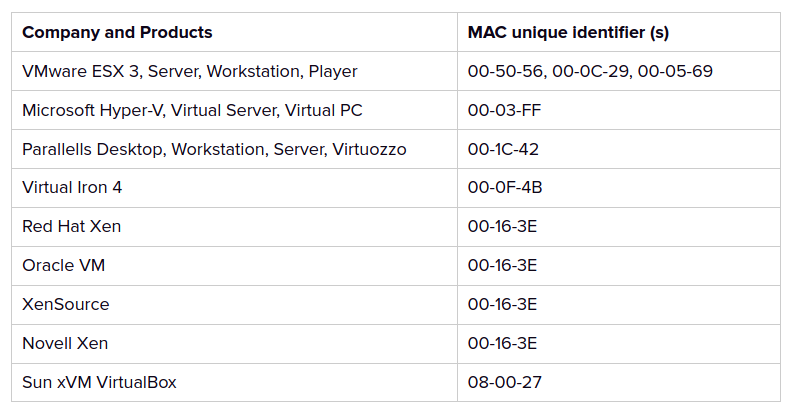
\includegraphics[width=\linewidth]{images/vms-mac-address.png}
\caption{Common VMs mac addresses \newline \url{https://www.techrepublic.com/blog/data-center/mac-address-scorecard-for-common-virtual-machine-platforms/}}
\label{fig:vms}
\end{figure}

Other execution artifacts are specific Registry Keys such as \textit{SystemBiosVersion} which takes the following values in VirtualBox and QEMU:
\begin{itemize}
    \item \begin{lstlisting}
        HARDWARE\Description\System (SystemBiosVersion) (VBOX)
    \end{lstlisting}
    \item \begin{lstlisting}
        HARDWARE\Description\System (SystemBiosVersion) (QEMU)
    \end{lstlisting} 
\end{itemize}

System files and drivers such as, among the others:
\begin{itemize}
    \item \begin{lstlisting}
        system32\drivers\vmci.sys
    \end{lstlisting}
    \item \begin{lstlisting}
        system32\drivers\VBoxVideo.sys
    \end{lstlisting}
    \item \begin{lstlisting}
        system32\vboxtray.exe
    \end{lstlisting}
\end{itemize}
Moreover other structures like ACPI tables, SMBIOS strings as well as Disk Size and RAM Size can be used to fingerprint the system and reveal the presence of a virtual machine. 


\section{Virtualization artifacts in QEMU}
QEMU due to its nature is one of the virtualization systems with the lowest footprint on the guest. Taken directly from the Al-Khaser github repository\footnote{\url{https://github.com/LordNoteworthy/al-khaser}} the artifacts used to fingerprint QEMU are the following:

\begin{itemize}
    \item \begin{lstlisting}[breaklines]
        HARDWARE\DEVICEMAP\Scsi\Scsi Port 0\Scsi Bus 0\Target Id 0\Logical Unit Id 0 (Identifier) (QEMU)
    \end{lstlisting}
    \item \begin{lstlisting}
        HARDWARE\Description\System (SystemBiosVersion) (QEMU)
    \end{lstlisting}
    \item \begin{lstlisting}
        SetupAPI SetupDiEnumDeviceInfo (GUID_DEVCLASS_DISKDRIVE)
    \end{lstlisting}
    \item \begin{lstlisting}
        SMBIOS string checks (Qemu)
    \end{lstlisting}
    \item \begin{lstlisting}
        ACPI string checks (Qemu)
    \end{lstlisting}
    \item \begin{lstlisting}
        qemu-ga.exe (QEMU)
    \end{lstlisting}
\end{itemize}

as well as the above mentioned \textit{CPUID} which will return specific strings both for QEMU alone or if used in combination with KVM.


\section{Testing frameworks}

There are available online different tools to perform automatic checks of the environment which aims to stress test the machine and verify how hidden is the analysis environment. The two most famous ones are Al-Khaser and Paranoid Fish\footnote{\url{https://github.com/a0rtega/pafish}}. Those tools are based on real techniques employed by malware to detect sandboxes and analysis environment and will run all the tests in sequence producing a final report of the passed and failed tests.

Paranoid Fish is a slightly older project which appears not to be maintained anymore while Al-Khaser is the evolution of Paranoid Fish and features many more techniques. It is important to note that not all the implemented techniques are a reliable indicator of the presence of a Virtual environment. Some checks such as the disk size, number of cores or the ram size might still fail even on computers still in use today. 